\chapter{LDAPによるユーザデータベース}

メールシステムに関連するデータの何かを、LDAPという外部データベースに置くとすれば、まず考えられるのはメールアドレスとユーザアカウントの情報でしょう。
本章では、LDAPでユーザアカウントを管理するときの考え方について、説明をします。

\section{なぜLDAPをユーザデータベースに使うのか}

ユーザアカウント管理を抽象化するとき、RDBMSやNoSQLでなく、LDAPを使用することが多いです。MicroSoftのActive Directoryも、リソース管理にLDAPを使用しています。
では、LDAPをユーザデータベースに使う理由は何でしょうか。

\subsection{LDAPと組織図の親和性}

\begin{figure}[htbp]
	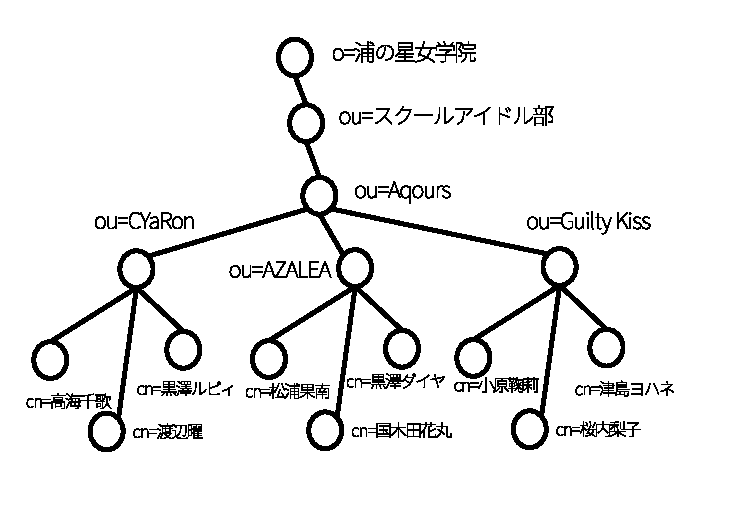
\includegraphics[width=12cm,clip]{draw/unitmap.eps}
	\caption{スクールアイドル部組織図}
	\label{fig:unitmap}
\end{figure}

一般に、組織図は木構造を取ります。その場合、ユーザは、木構造のリーフノードとして置かれます。このような構造をそのまま表すには、木構造データベースであるLDAPが適しています。
たとえば、スクールアイドル部という部署で、ユニットが三つあります。各ユニットには、3人ずつメンバーがいます。
この場合、図\ref{fig:unitmap} スクールアイドル部をルートノードにした、木構造であらわすことができます。

この程度なら、RDBMSでも、一対多の関連があるテーブルの連鎖で表すことができるでしょう。
ですが、ユーザアカウントを検索するとき、どこのユニットに属しているかという情報なしで、探す必要があります。そのようなときに、LDAPであれば、スクールアイドル部以下の子ノードを、再帰的に探索するだけです。
一方、SQLのSELECT文で探索を行うのは面倒です。三つのユニットの空間をUNIONして探すとしても、各ユニットの属性が揃っている必要があります。

\subsection{構造の自由度}

\begin{figure}[htbp]
	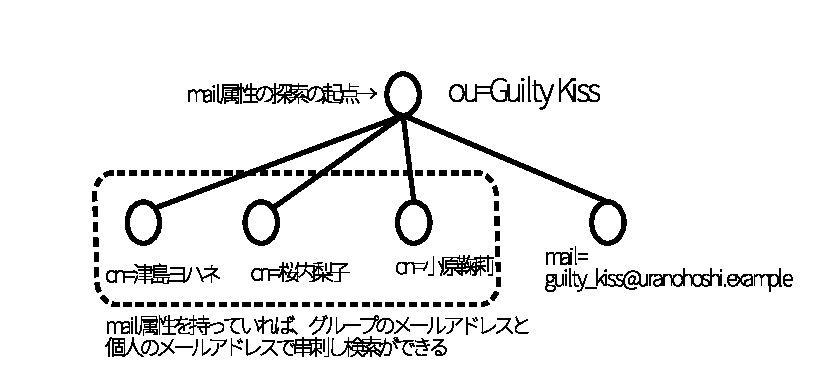
\includegraphics[width=12cm,clip]{draw/nodesearch.eps}
	\caption{構造の自由度}
	\label{fig:nodedn}
\end{figure}

LDAPは、ある親ノードの下にある子ノードに、何を置いてもかまいません。先ほどの例では、ユニットの下にメンバーのノードを置いていました。
図\ref{fig:nodedn}にあるように、
このノードと一緒に、ユニットの代表メールアドレスの情報をDNとして持つノードを置くこともできます。

それだけだと性質の違うノードをおけるだけのように思えます。ですが、LDAPの場合は、属性が同じであればこの両者を一度に検索対象とすることができます。

たとえば、ユニットのメンバーのノードと、代表メールアドレスのノードが、それぞれ同じ属性mailを持っているとします。このとき、あるメールアドレスがユニットのメンバーもしくは代表メールアドレスであるかを調べたい場合、ユニットの子ノードすべてを検索対象として、mail属性に該当の者があるかを検索すればよいことになります。


\subsection{LDAP探索の計算量}

\begin{figure}[htbp]
	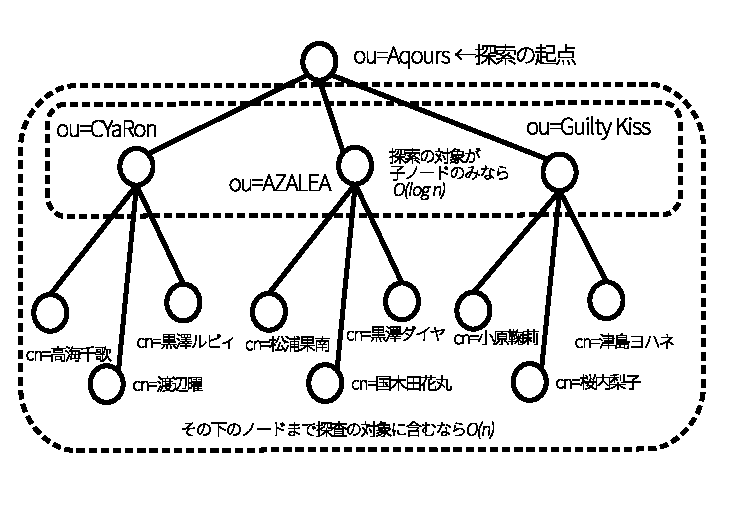
\includegraphics[width=12cm,clip]{draw/order.eps}
	\caption{探索の計算量}
	\label{fig:order}
\end{figure}

LDAPは、DNによってあるノードを指定し、そのノードの子ノードを検索対象とする、もしくは、その子ノード以下を再帰探索の対象とするという探し方をします。
このとき、指定したノードの子ノードを探索対象とする場合の計算量は、$O(\log n)$という特徴があります。共通の親を持つ兄弟ノードの中から検索するとき、計算量がいつも同じです。

一方、その兄弟ノードがそれぞれ子となるノードを持っており、その兄弟ノードの子ノードも探索の範囲であった場合、再帰探索がおこなわれます。このときの計算量は、$O(n)$になります。

LDAPで検索を行うときは、検索対象となるノードがどこにあるかに当たりを付け、なるべくその親を起点にするというのが、基本的な戦略になります。

\subsection{書き換え頻度}

LDAPは、頻繁な書き換えには向かない、という欠点があります。木構造であるということは、その構造そのものを書き換えるにはコストがかかります。また、データもハッシュテーブルであるBerkeleyDBをバックエンドにしている実装もあり、書き換えのパフォーマンスはあまり高くありません。

ですが、ユーザアカウントデータベースは、書き換え頻度が少ないという特徴があります。そのため、RDBMSほどの書き換えパフォーマンスは必要なく、LDAPを使う上での問題にはなりません。

\section{LDAPのノード}

LDAPのノードは、一つ以上の属性を含みます。その属性の取捨選択は、どのように行うのでしょうか。

スキーマという属性のセットをノードごとに選択することで

\subsection{属性と属性値}

\begin{figure}[htbp]
	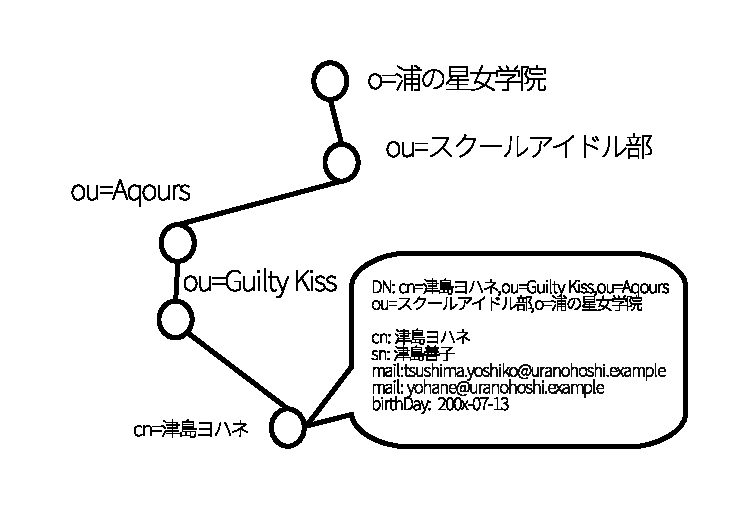
\includegraphics[width=12cm,clip]{draw/attribute.eps}
	\caption{属性と属性値}
	\label{fig:attribute}
\end{figure}

属性は、ノードが持つ情報です。その属性に対応した値が、属性値となります。
図\ref{fig:attribute}では、リーフノードに含まれる属性と、その属性値を例として示しています。
このノードは人の情報を表すので、名前、メールアドレス、誕生日、注釈を含むノードとしています。
属性は全てのノードがもちます。このノードのDNに含まれるcn=津島ヨハネも、属性です。
そのため、LDAPのノードは、最低限ひとつの属性と、その値を持っていることになります。\footnote{実際には後述するオブジェクトタイプを指定するための属性も含める必要があります。}

ひとつの属性は、その値としての属性値をひとつ取ります。例えば、mailという属性は、メールアドレスをひとつその属性値として取ります。複数のメールアドレスを、その属性値としてることはありません。

属性は、ひとつのノードにひとつしか置けないものと、複数置くことができるものとがあります。これは、後述する属性の定義によります。たとえば、ユーザアカウント情報のノードでは、ユーザ名はひとつしか採ることができないように定義します。その一方、メールアドレスは、複数採ることができるように定義します。

もし、ひとつのノードに情報としての属性値を複数持たせたいときは、同じ属性を複数持たせます。たとえば、あるユーザアカウントが、メール8アドレスをtsushima.yoshiko@uranohosi.exampleとyohane@uranohoshi.exampleの二つ持っていれば、mail属性を二つ持つノードとして設定します。そうすることで、複数のメールアドレスをひとつのユーザアカウントの情報として持たせます。

\subsection{LDIF}

LDAPのノードを定義するためには、テキスト形式で情報を定義します。この形式を、LDIF(LDAP Data Interchange Format)と呼びます。LDIF形式は、LDAPからエントリをダンプするときにも使用されます。

LDIFは、LDAPのノードのエントリに含まれる情報を、ノードがルートに近い、もしくは、再起探索の順番で描いたものです。あるノードのDNは、その親となる上位のノードが定義済みでなければなりません。そのため、ルートに近いところから、あるいは、再帰探索の順番でエントリが並べられます。

また、LDIFでは、UTF-8はBase64エンコードされます。以下の例では、UTF-8の部分は、プレーンテキストのままで記述しています。
図\ref{fig:attribute}の内容をダンプしたものを示します。
\begin{verbatim}
dn; o=浦の星女学院
changeType: add
objectClass: organizationalUnit
o: 浦の星女学院

dn; ou=スクールアイドル部,o=浦の星女学院
changeType: add
objectClass: organizationalUnit
ou: スクールアイドル部

dn; ou=Aqours.ou=スクールアイドル部,o=浦の星女学院
changeType: add
objectClass: organizationaUnit
ou: Aqours

dn; ou=Guilty Kiss,ou=Aqours.ou=スクールアイドル部,o=浦の星女学院
changeType: add
objectClass: organizationaUnit
ou: Guilty Kiss

dn; cn=津島ヨハネ,ou=Guilty Kiss,ou=Aqours.ou=スクールアイドル部,o=浦の星女学院
changeType: add
objectClass: person
cn: 津島ヨハネ
sn: 津島良子
\end{verbatim}

\subsection{オブジェクトクラス}

あるノードがどのような属性を含むかは、オブジェクトクラスという属性セットを選択することで決まります。この属性セットは、ひとつ、もしくは複数設定することができます。また、オブジェクトクラスはノードごとに選択します。

あるノードが使用するオブジェクトクラスは、属性objectClassの属性値として定義されます。objectClassは、一つのノードで複数現れてもかまわない属性です。

代表的なオブジェクトクラスとして、inetOrgPersonがあります。このスキーマは、ユーザアカウント情報に必要な、属性値のセットを含んでいます。
また、ミドルウェアやアプリケーションで、専用の属性を追加するためのオブジェクトクラスを追加するためのファイルが添付されていることがあります。
例として、Courier-IMAPは、専用のオブジェクトクラスの定義ファイルを、ソースツリーに添付しています。


\subsection{スキーマ}
LDAPでスキーマと呼ばれるのは、オブジェクトクラスの定義です。スキーマを読み込ませることで、そのDITで使用可能なオブジェクトクラスが定義されます。
この定義はテキストで記述され、、スキーマファイルと呼ばれます。このスキーマファイルは、以下のように記述されています。

\begin{verbatim}
attributeType( 2.5.4.41 NAME 'name'
DESC 'name(s) associated with the object'
EQUALITY caseIgnoreMatch
SUBSTR caseIgnoreSubstringsMatch
SYNTAX 1.3.6.1.4.1.1466.115.121.1.15{32768} )
attributeType( 2.5.4.3 NAME ( 'cn' 'commonName' )
DESC 'common name(s) assciatedwith the object'
SUP name )
\end{verbatim}

スキーマファイルは、LDAPサーバに添付されているものと、ミドルウェアなどが独自に使用するために添付されているものとがあります。


\subsection{OID}

スキーマファイルの中で、2.5.4.41や、1.3.6.1.4.1.1466.115.121.1.15という数字の列が現れています。これは、OID(Object ID)と呼ばれる、オブジェクトを一意的に識別するためのものです。ANSIで管理されています。

これは、LDAPが、ITU-Tで定義されたディレクトリサービスを簡易化した実装であることに撚ります。いわば、昔のディレクトリ定義の名残を引きずっている部分です。

SNMPで使うときなど、OIDはデバイスを抽象的に表現するためにも使われます。この場合は、MIB(Management Information Base)と呼びます。

2.5.4というのはディレクトリサービスの属性であることを著わすために定義されているOIDです。その後の数字が、何を表す属性だえるかを著わすIDとなっています。また、1.3.6.1.4.1というのは、この次に、プライベートな組織を著わすIDが置かれます。そして、その先のIDは、その組織で自由に定義してよいことになっています。
この組織のIDを、PEN(Private Enterprise Number)と呼びます。PENが1466は、これ以降でデータの形式を定義するのに使われるOIDです。

1.3.6.1.4.1.(PEN)というOIDを、プライベートMIBと呼びます。これは主にSNMPでの呼び方でアリ、プライベートに定義され、他のOIDとかぶらないことが保証されたたOIDであると考えて構いません。また、OIDのかぶりを避けるため、独自にOIDを定義するときは、PENを取得する必要があります。
PENは、IANAに申請すれば無料で取得可能です。
独自のスキーマを作成するときは、OIDとして1.3.6.1.4.1.(PEN)ではじまるOIDを割り当てるようにします。





\section{アクセスコントロール}

\begin{figure}[htbp]
	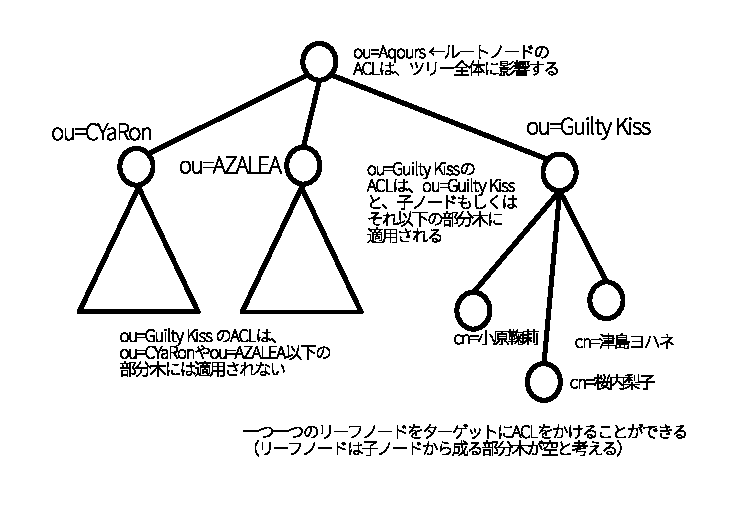
\includegraphics[width=12cm,clip]{draw/acl.eps}
	\caption{LDAPのアクセスコントロール}
	\label{fig:acl}
\end{figure}

LDAPのアクセスコントロールは、どのような概念なのでしょうか。それは、部分空間内のノードに対して、誰にどのようなアクセスを許可するか、という概念です。慣例的に、Access Control Listを略したACLと書かれることがあります。
LDAPのアクセス権は、図\ref{fig:acl}にあるように、あるノードを起点として、そのノード、そのノードを起点とする部分木を単位として適用されます。

ルートノードにACLを適用した場合、そのACLはLDAPツリー全てに影響します。これは、ルートノードを起点とした部分木とは、その木の全体であるためです。
それとは逆に、ACLは、リーフノードにも適用可能です。リーフノードは、子ノードや更にその子ノードからなる部分木が空であると考えます。そうすることで、LDAPのアクセスコントロールは、あるノードを起点とした部分木に対して適用される、という一貫性を持たせています。



\subsection{LDAPアクセスとbind}

LDAPのノードにアクセスするときは、bindによるアクセスと、匿名アクセスの二つの概念があります。

bindは、LDAPクライアントがDITの情報を参照するときに、そのDITに含まれるユーザ情報とパスワードで認証をすることです。このユーザ情報は、DITの中のどこにおいても構いません。このように、LDAPで認証を行ない、アクセスとユーザを紐付けるうことを、bindといいます。
アクセス制御を行うときは、bindをすることが前提となります。

匿名アクセスは、あるDITの情報を参照するときに、何らかの認証を行わずに、アクセスすることです。つまり、bindせずにアクセスする場合となります。匿名アクセスは、ユーザ認証にLDAPのサービスを利用する場合など、LDAPのクライアントとなる系がbindに対応していない場合など、限られた場合に用いるようにします。


\subsection{アクセス権とスコープ}

LDAPのアクセスコントロールは、あるノード基準にして、その子ノード、もしくは、それ以下の部分木に再帰的に適用します。
つまり、LDAPのアクセス権のスコープは、部分空間がその単位になります。

OpenLDAPであれば、slapd.conf(5)で、以下のようにアクセスコントロールを設定します。このルールは、上から順番にチェックしていって、一番最初に適用されたものが適用される、ファーストマッチになります。

\begin{verbatim}
access to アクセス制御の対象となるDN
    by アクセス制御の対象条件 アクセス権
    by アクセス制御の対象条件 アクセス権
......

access to アクセス制御の対象となるDN
    by アクセス制御の対象条件 アクセス権
    by アクセス制御の対象条件 アクセス権
......
\end{verbatim}

アクセス許可の条件には、DNやIPアドレスなどを用います。たとえば、DN:ou=users,ou=uranohoshi,ou=exampleの子ノードの情報を使って、誰でも認証の結果を受け取ることができる、というACL設定です。

\begin{verbatim}
access to dn.children="ou=users,dc=uranohoshi,dc=example"
    by anonymous auth
\end{verbatim}

アクセス制御の対象として、属性まで絞り込むことができます。このときは、attasというディレクティブを追加して、アクセス制御する属性を記述します。今度は、自分のアカウントに限ってパスワードを変更できるように記述します。
その次のアクセス権設定は、パスワード以外の属性は、自分のものを読むだけ、という設定です。

\begin{verbatim}
access to dn.children="ou=users,dc=uranohoshi,dc=example"
    attrs=userPassword
    by self write

access to dn.children="ou=users,dc=uranohoshi,dc=example"
    by self read
    by * none
\end{verbatim}

\subsection{アクセス対象}

LDAPのアクセス権を設定する対象をどのように設定するかについて、説明します。

\paragraph{anonymous}
匿名でアクセスしている状態を指定します。全てのアクセスのデフォルトで、anonymousのアクセス許可は設定されていません。

\paragraph{•}
ワイルドカードで、bindしているアカウント全てを指定します。anonymousは含まれません。

\paragraph{self}
アクセス対象となっているノードがユーザアカウントの情報を思っており、そのユーザとパスワードでbindしている場合を指定します。たとえば、自分のパスワード変更を許可する場合に指定します。

\paragraph{dn.children="DN"}
指定したDNか、その子ノードのいずれかでbindしていることが条件となります。DNは、ダブルクオーテーションでかこんで、記述します。

\paragraph{dn.subtree="DN"}
指定したDNか、それ起点とした部分木に含まれるノードのいずれかでbindしていることが条件となります。DNは、ダブル区オー手ションで囲んで記述します。

\subsection{LDAPのアクセス権}

LDAPへのアクセス権には、どのようなものがあるのでしょうか。主なものを、OpenLDAPでの設定値を併記して節瞑していきます。

\paragraph{none}
アクセス許可しないということです。条件に一致する場合、DN以下の部分区間に対してアクセスを許可しません。

\paragraph{auth}
DN以下の情報を用いて、認証を行ない、結果を取得することを許可します。

\paragraph{continue}
属性値を比較して、その結果を取得することを許可します。

\paragraph{search}
属性値の検索を行うことを許可します。

\paragraph{read}
ノードの読み取りを許可します。そのノードに含まれる属性値の、比較や検索を行うこともできます。

\paragraph{write}
readのアクセス権にくわえて、DNで指定したノードの書き換えも許可します。

\paragraph{continue}
ACL設定は基本的にファーストマッチです。ですが、マッチした場合のアクセス権を維持して、次の条件をチェックしたい場合もあります。このときは、アクセス権の跡にcontinueと追記します。
continueで次の条件に行き、その条件にマッチした場合、その次の行のACLが適用されます。

以下の例は、bindしていても、ou=aqours以下の部分木へのアクセスは許可しません。ですが、管理アカウントでアクセスしているときは、アクセスが許可されます。

\begin{verbatim}
access to dn.children="ou=aqours,dc=uranohoshi,dc=example"
    by * none continue
    by dn.children="cn=Manager,dc=uranohoshi,dc=example" write

\end{verbatim}